\documentclass{scrreprt}
\usepackage[english]{babel}
\usepackage[T1]{fontenc}
\usepackage{lmodern}
\usepackage{blindtext}
\usepackage[utf8]{inputenc}
\usepackage{siunitx} %For unit handling%
\renewcommand{\familydefault}{\sfdefault}
\newcommand{\unit}[1]{\ensuremath{\, \mathrm{#1}}}
\usepackage{amssymb, amsmath, cancel, ulem, graphicx, float, tabularx, multirow, bm}
\usepackage{amsmath}
\usepackage{caption}
\usepackage{subcaption}
\usepackage{mathtools}
\usepackage{tikz}
\usepackage{commath}
\usepackage{nameref}
\newcommand*\circled[1]{\tikz[baseline=(char.base)]{
            \node[shape=circle,draw,inner sep=1pt] (char) {#1};}}
\renewcommand{\phi}{\varphi}


\setcounter{secnumdepth}{5}
\setcounter{tocdepth}{5}

\author{Urs Gerber\\09-921-156 \and Gian-Luca Mateo\\11-113-545}
\date{23th of May 2013}

\title{Molar Heat Capacity}
\subtitle{Practical course report}

\begin{document}

\maketitle

\tableofcontents
\newpage

\chapter{Experiment: Molar Heat Capacity}
\section{Introduction}


\subsection{Goal of the experiment}
The goal of this experiment is to experimentally determine the ratio $\gamma = \frac{C_v}{C_p}$ of the molar heat capacity for constant volume to the molar heat capacity for constant pressure for different gases, namely Argon ($Ar$), Nitrogen ($N_2$) and Carbon Dioxide ($CO_2$). 
 
\subsection{Theory} 
The state of an ideal gas can be manipulated by adding or removing heat or work to/from the system. Two parameters can define the way a gas behaves under such manipulations, namely how much energy is needed to heat a gas for constant volume and how much energy is needed to heat it for constant pressure.
\begin{equation}
C_v = \left. \frac{\delta Q}{\dif{T}} \right\|_{V=const}
\qquad C_p = \left. \frac{\delta Q}{\dif{T}} \right\|_{p=const} 
\end{equation}
...
\
\subsubsection{Error analysis}


\section{Experiment setup and execution}

\subsection{Used materials}
The materials used in this experiment are the following:
\begin{itemize}
\item A gas tank made of glass, $V = 5633 \unit{cm^3}$
\item A tube attached vertically to the glass, $L \approx 45\unit{cm}$, $R = 16 \unit{mm}$
\item A small metal ball, $m = 17 \unit{g}$
\item 3 gas bottles, containing $N_2$, $CO_2$ and $Ar$ respectively
\end{itemize}

\subsection{Assembly and Execution}

\section{Measurements}
\begin{figure}[H]
	\centering
  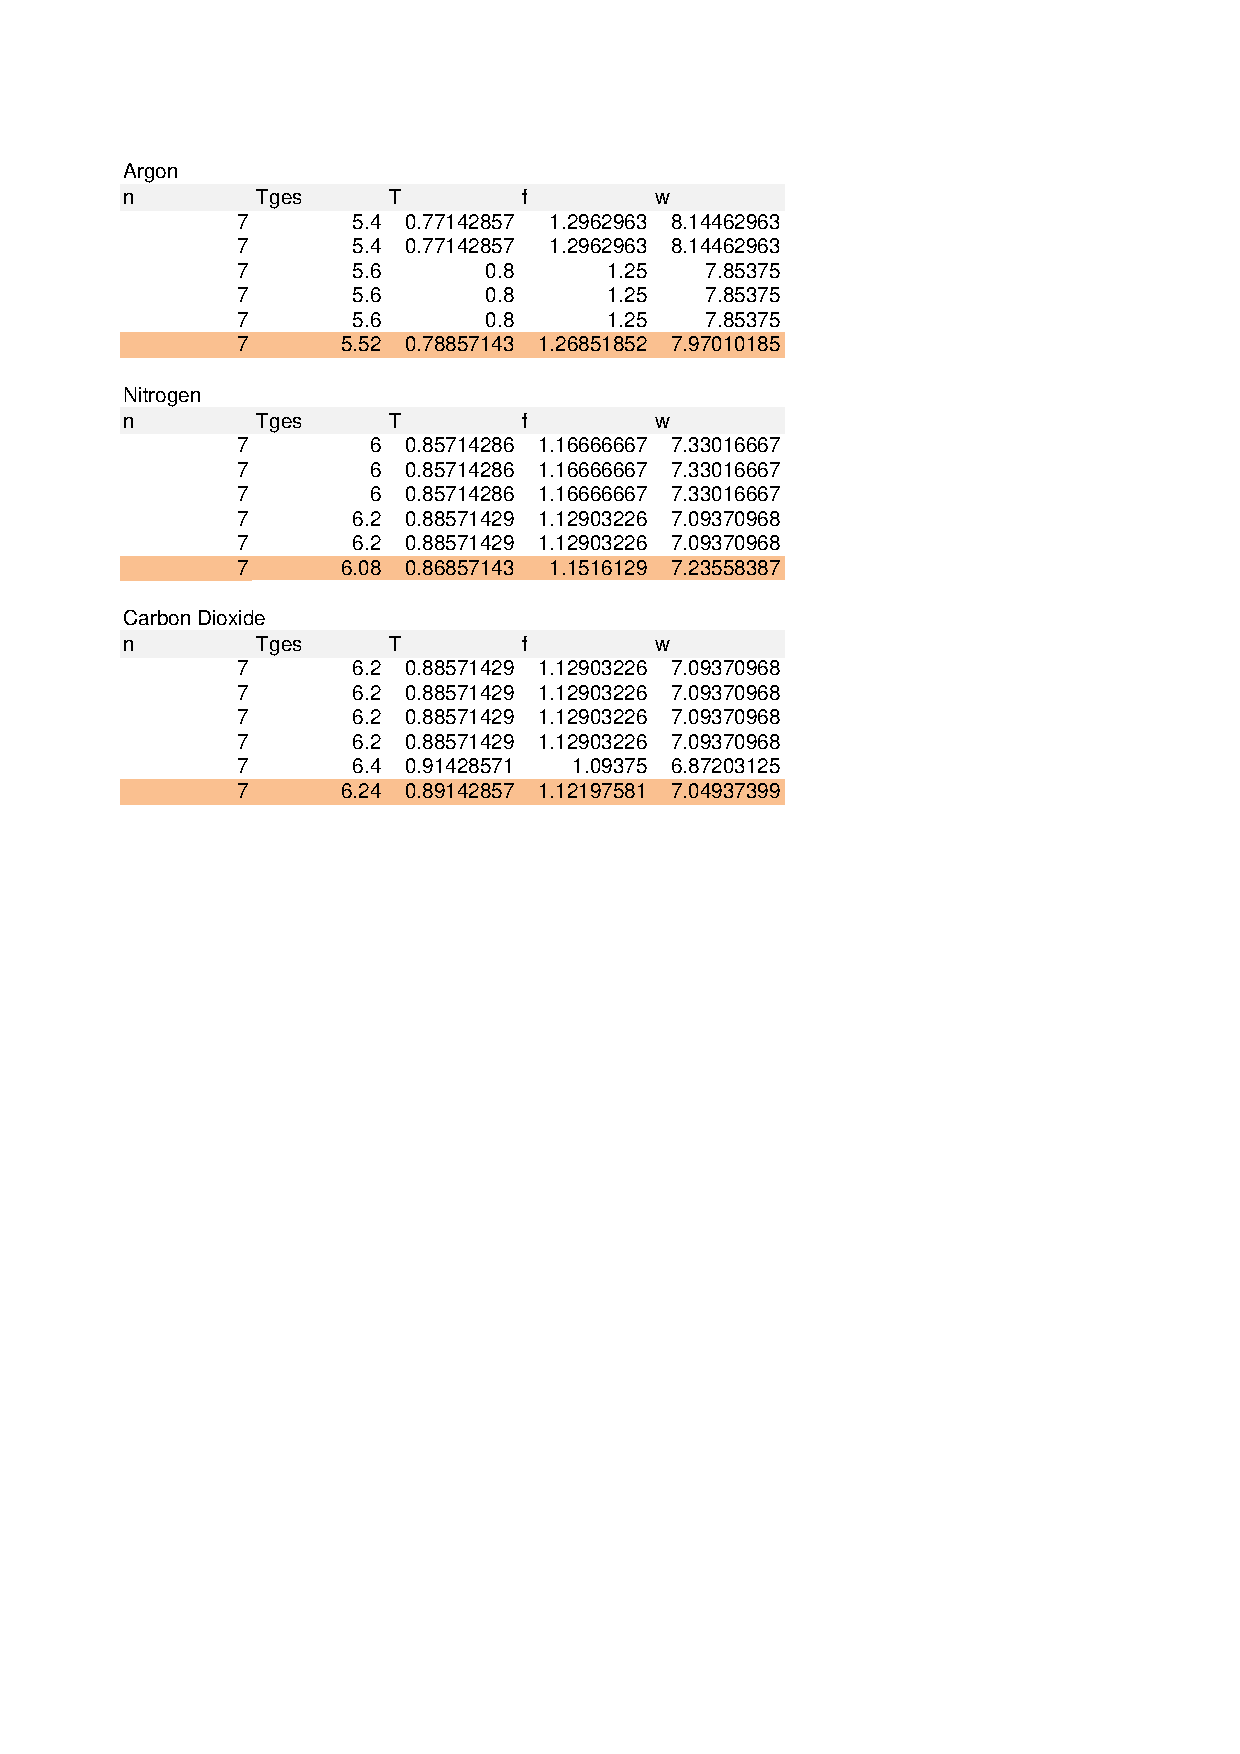
\includegraphics[width=0.7\textwidth]{diag/rawvals.pdf}
	\caption{Measured Values for the Oscillation Period of the Ball}
	\label{fig:measurement}
\end{figure}

\begin{figure}[H]
	\centering
  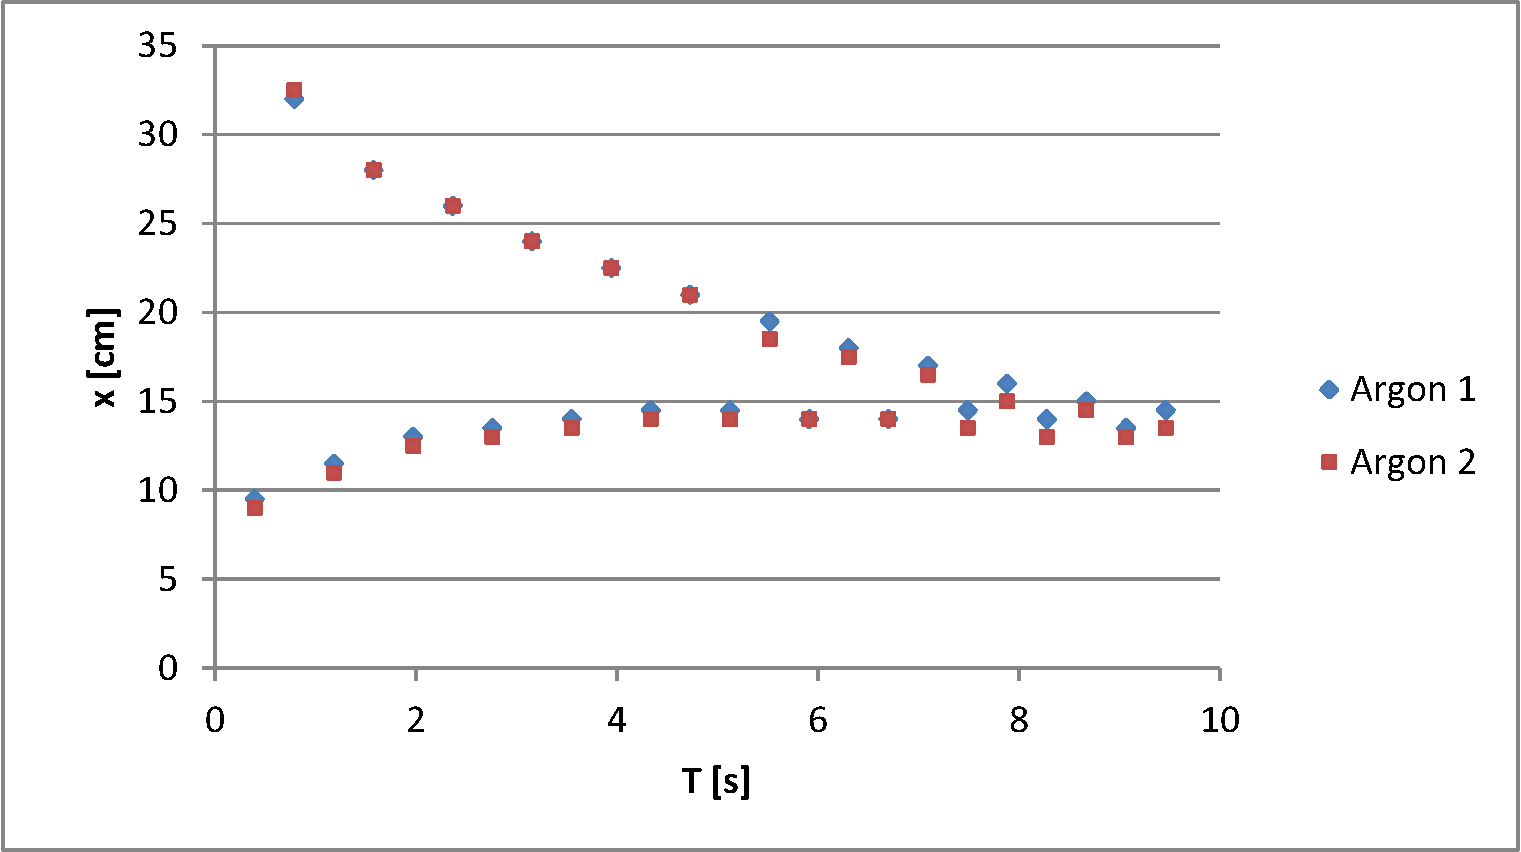
\includegraphics[width=0.7\textwidth]{diag/argon.pdf}
	\caption{Measured Oscillations of the Ball with Argon in the Tank}
	\label{fig:argon}
\end{figure}

\begin{figure}[H]
	\centering
  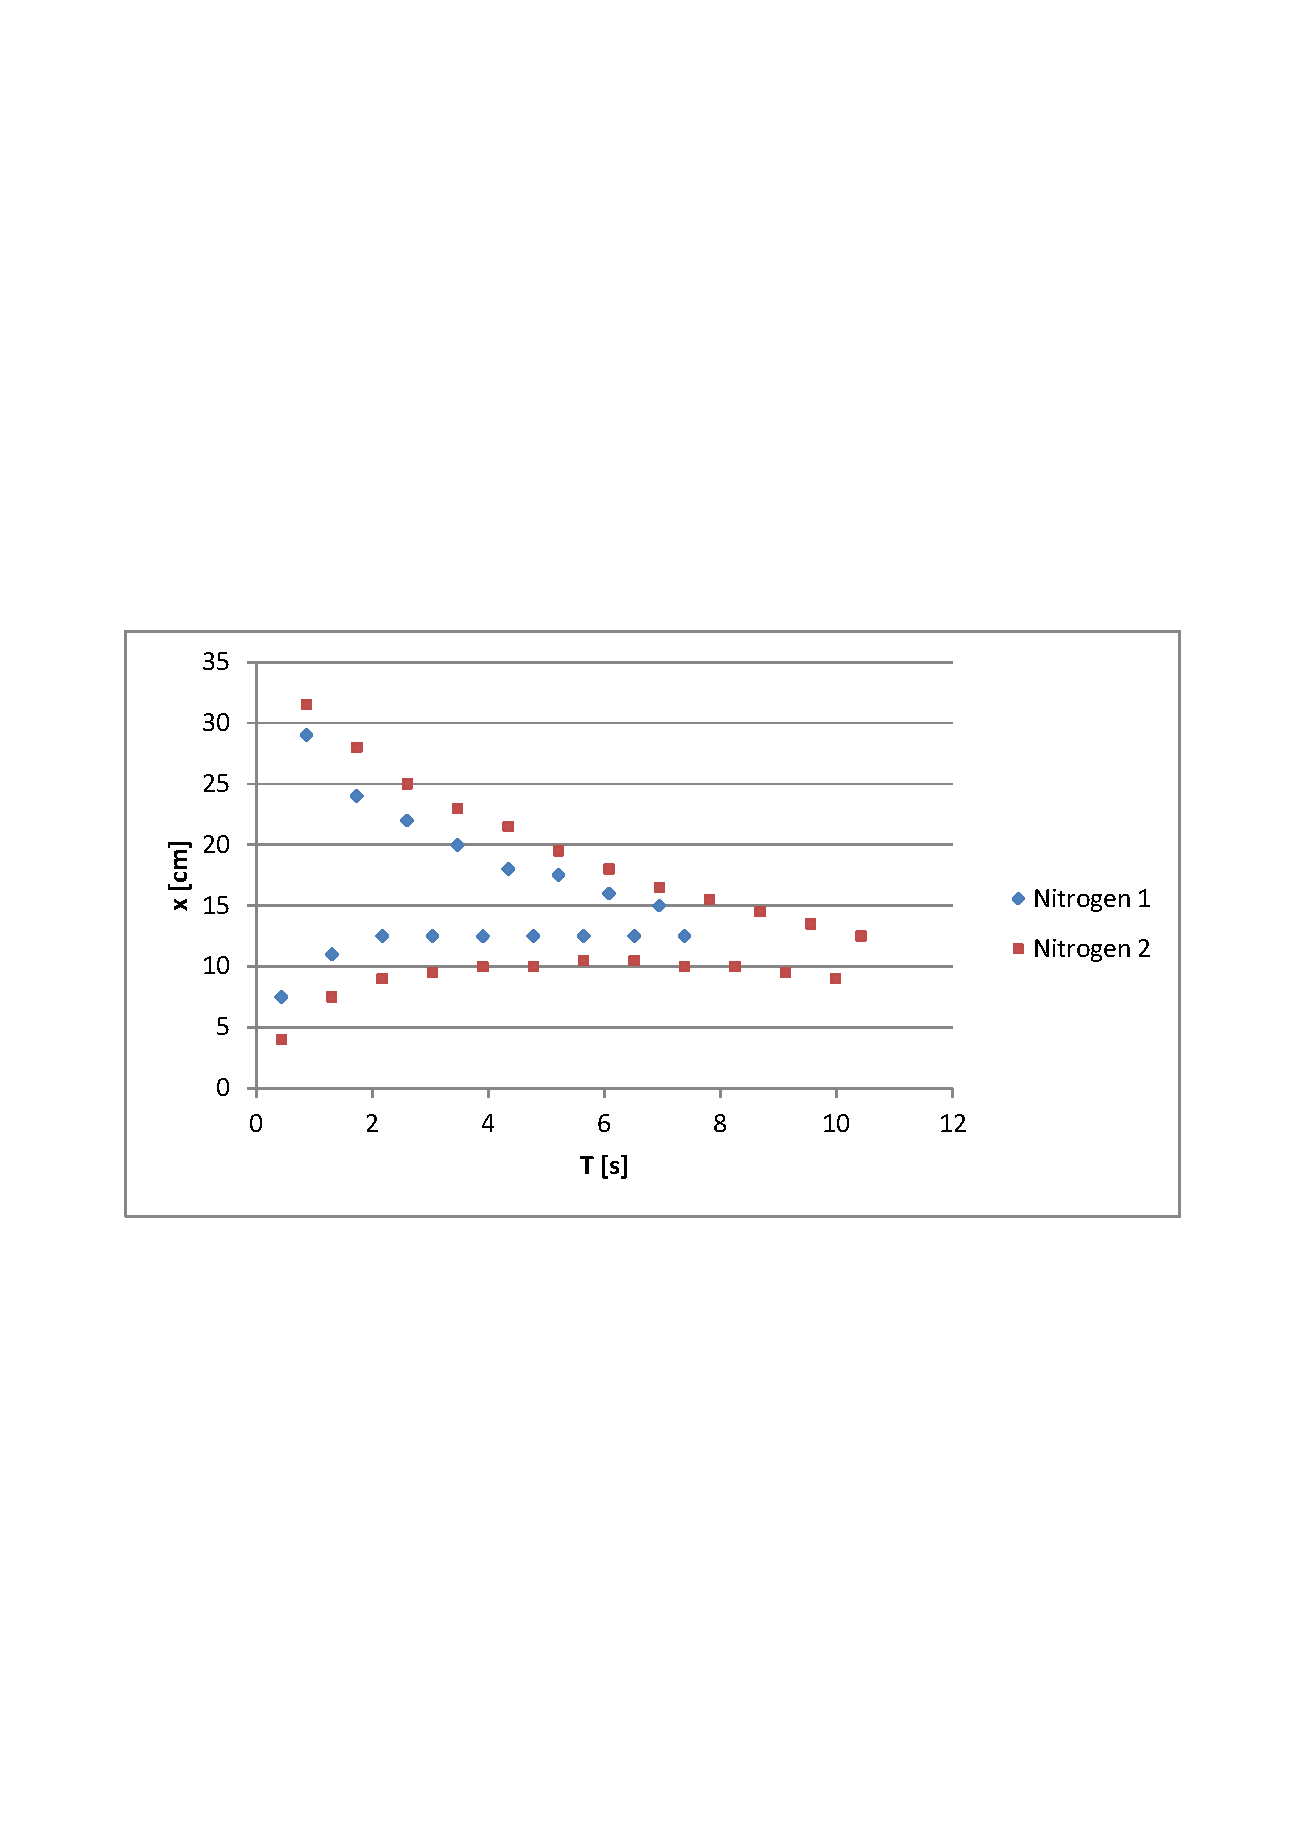
\includegraphics[width=0.7\textwidth]{diag/nitrogen.pdf}
	\caption{Measured Oscillations of the Ball with Nitrogen in the Tank}
	\label{fig:nitrogen}
\end{figure}

\begin{figure}[H]
	\centering
  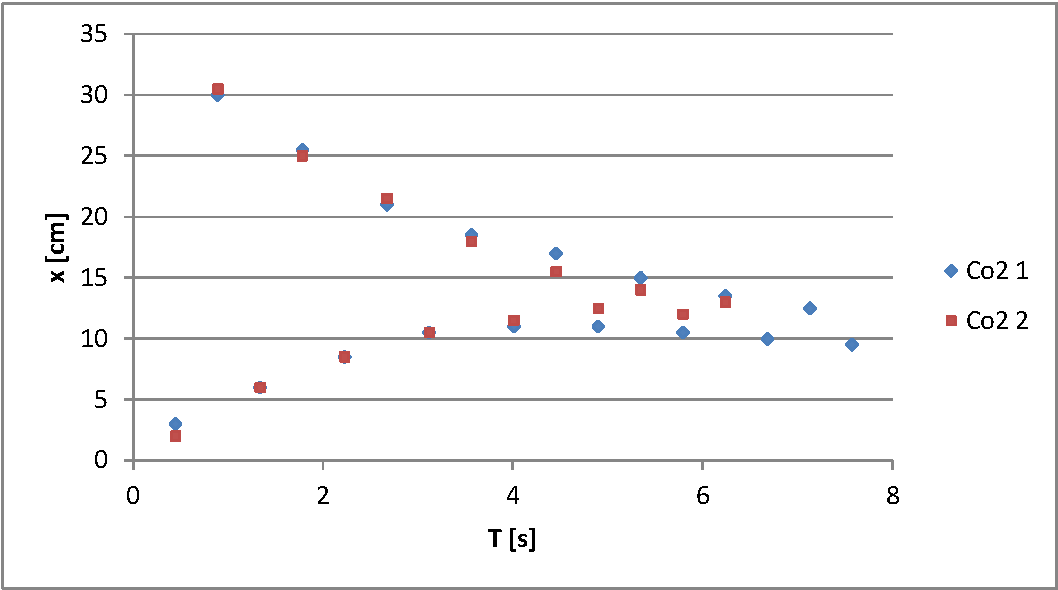
\includegraphics[width=0.7\textwidth]{diag/co2.pdf}
	\caption{Measured Oscillations of the Ball with Carbon Dioxide in the Tank}
	\label{fig:co2}
\end{figure}


\section{Analysis and Discussion}

\subsection{Sources of error}
\label{sec:error}


\section{Conclusion}


\begin{thebibliography}{9}

\bibitem{physcript13}
  Peter Wurz,
  \emph{Anleitung zum Physikpraktikum}
  FS2013

\end{thebibliography}

\end{document}
